\documentclass[10pt]{beamer}

\usetheme{metropolis}
\usepackage{appendixnumberbeamer}

\usepackage{booktabs}
\usepackage[scale=2]{ccicons}

\usepackage{pgfplots}
\usepgfplotslibrary{dateplot}

\usepackage{listings}
\lstset{language=R}

\usepackage[utf8]{vietnam}

\usepackage{color}
\definecolor{mygreen}{rgb}{0,0.6,0}
\definecolor{mygray}{rgb}{0.5,0.5,0.5}
\definecolor{mymauve}{rgb}{0.58,0,0.82}

\lstset{ %
  basicstyle=\footnotesize,        % the size of the fonts that are used for the code
  breakatwhitespace=false,         % sets if automatic breaks should only happen at whitespace
  breaklines=true,                 % sets automatic line breaking
  captionpos=b,                    % sets the caption-position to bottom
  commentstyle=\color{mygreen},    % comment style
  deletekeywords={...},            % if you want to delete keywords from the given language
  escapeinside={\%*}{*)},          % if you want to add LaTeX within your code
  extendedchars=true,              % lets you use non-ASCII characters; for 8-bits encodings only, does not work with UTF-8
  frame=single,	                   % adds a frame around the code
  keepspaces=true,                 % keeps spaces in text, useful for keeping indentation of code (possibly needs columns=flexible)
  keywordstyle=\color{blue},       % keyword style
  language=Octave,                 % the language of the code
  otherkeywords={*,...},           % if you want to add more keywords to the set
  numbers=left,                    % where to put the line-numbers; possible values are (none, left, right)
  numbersep=5pt,                   % how far the line-numbers are from the code
  numberstyle=\tiny\color{mygray}, % the style that is used for the line-numbers
  rulecolor=\color{black},         % if not set, the frame-color may be changed on line-breaks within not-black text (e.g. comments (green here))
  showspaces=false,                % show spaces everywhere adding particular underscores; it overrides 'showstringspaces'
  showstringspaces=false,          % underline spaces within strings only
  showtabs=false,                  % show tabs within strings adding particular underscores
  stepnumber=1,                    % the step between two line-numbers. If it's 1, each line will be numbered
  stringstyle=\color{orange},     % string literal style
  tabsize=2,	                   % sets default tabsize to 2 spaces
  title=\lstname                   % show the filename of files included with \lstinputlisting; also try caption instead of title
}

\usepackage{xspace}
\newcommand{\themename}{\textbf{\textsc{metropolis}}\xspace}

\metroset{block=fill}

\title{Reproducible Research}
\subtitle{}
\date{18 March 2016}
\author{
    \href{mailto:christopher.gandrud@city.ac.uk}{Christopher Gandrud}
}
\institute{SG1022, City University London}
% \titlegraphic{\hfill\includegraphics[height=1.5cm]{logo.pdf}}

\begin{document}

\maketitle

\begin{frame}{Table of contents}

    \begin{itemize}
        \item \textbf{What} is research?

        \item \textbf{What} is reproducible research?

        \item \textbf{Why} do we need reproducible research

        \item \textbf{How} to do really reproducible research
    \end{itemize}

\end{frame}

\section{What is reproducible research?}

\begin{frame}{What is research?}

    \begin{center}
        {\large{\emph{Is this research?}}}

        \vspace{0.5cm}

        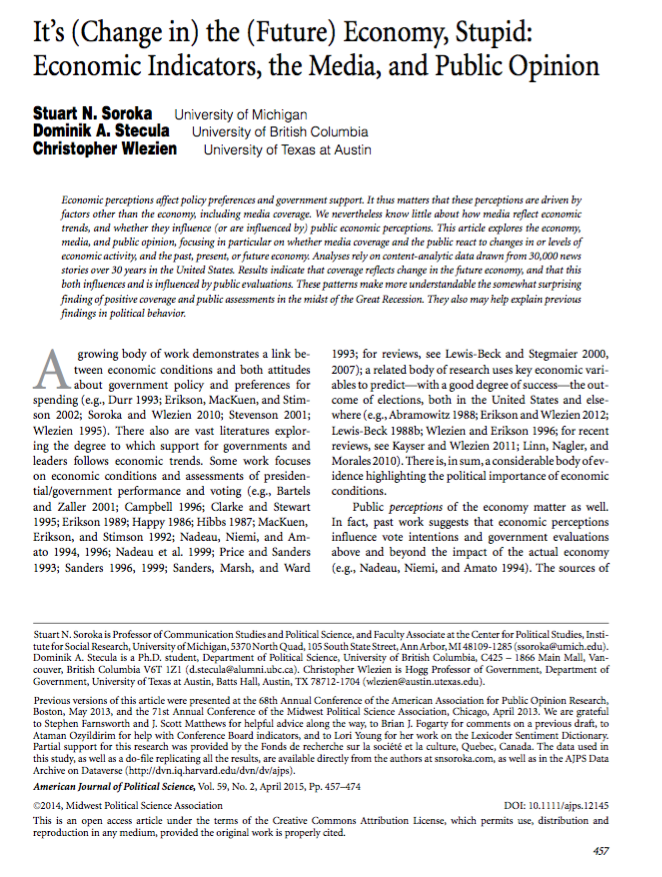
\includegraphics[scale=0.2]{img/journal_ss.png}
    \end{center}
\end{frame}

\begin{frame}{What is research?}

    \begin{center}
        {\large{\emph{Is this research?}}}

        \vspace{0.5cm}

        
\includegraphics[scale=0.2]{img/cox.png}
    \end{center}
\end{frame}

\begin{frame}{Are they research?}

    \begin{alertblock}{No}
        Papers, articles, slideshows, talks, books are the {\large{\textbf{advertising, not the research}}}.
    \end{alertblock}

\end{frame}

\begin{frame}{Are they research?}


    Papers, articles, slideshows, talks, books are the {\large{\textbf{advertising, not the research}}}.

    \vspace{1cm}

    \begin{block}{What are they?}
        \textbf{Presentation documents} \emph{announcing} select findings and \emph{trying} to convince us that they are correct (Mesirov 2010).
    \end{block}
\end{frame}

\begin{frame}{What is research?}

    Quantitative social science research involves the \textbf{procedures} and \textbf{choices} researchers make to gather data, process it, and analysis it in order to address their research questions.

    \vspace{1cm}

    For {\large{computational research}}, this includes ``the {\large{full software environment, code, and data}} that produced the results'' (Donoho 2010, 3015).

\end{frame}

\begin{frame}
    \begin{center}
        {\large{We need to make available our research, not just the advertising!}}
    \end{center}
\end{frame}


\section{What is reproducible research?}

\begin{frame}{Replicability}

    If we make the research available, not just the advertising, then it will be {\large{more likely}} that other researchers can replicate our work.

    \vspace{1cm}

    \begin{exampleblock}{Replicable Research}
        When there is \emph{sufficient information} available for \emph{independent researchers} to make the \emph{same findings}, using the \emph{same procedures} with \emph{new data}.
    \end{exampleblock}

\end{frame}

\begin{frame}{But\ldots}

    Sometimes full replications \textbf{are not feasible} because:

    \begin{itemize}
        \item \emph{limited resources} for gathering new data (e.g. very expensive to build another Large Hadron Collider),

        \vspace{0.5cm}

        \item the original research already \emph{sampled the universe} of cases.
    \end{itemize}

    \vspace{0.5cm}

    {\large{So\ldots}}

\end{frame}

\begin{frame}{Reproducibility}

    \begin{exampleblock}{Reproducible Research}
        When there is sufficient information available for independent researchers to make the same findings, using the same procedures with the \emph{same data}.
    \end{exampleblock}

\end{frame}

\begin{frame}{Reproducibility}

    \begin{exampleblock}{Really Reproducible Computational Research}
        ``\ldots the \textbf{data and code} used to make a finding are available and they are sufficient for an independent researcher to recreate the finding'' (Peng 2011, 1226)
    \end{exampleblock}

\end{frame}

\begin{frame}{Reproducible and Replicable}

    Reproducible research \textbf{enhances} replicability.

    \begin{itemize}
        \item Reproducible research is a precondition for replicable research.

        \vspace{0.5cm}

        \item Reproducibility is a `second best' if attempting a replication is not possible.

        \vspace{0.5cm}

        \item If it is \textbf{easy} to reproduce your work, more likely that someone else will be able to \textbf{replicate} it.
    \end{itemize}

\end{frame}

\begin{frame}{Reproducible and Replicable}

    \begin{alertblock}{Important!}
        ``\textbf{A study can be reproducible and still be wrong}'' (Peng 2014)

        \vspace{0.5cm}

        E.g. a finding that is statistically significant in one study may remain statistically significant when reproduced using the original data/code, but replication studies are unable to find a similar result.

        \vspace{0.5cm}

        The original finding could just have been \textbf{noise}.
    \end{alertblock}

\end{frame}

\section{Why reproducible research?}

\begin{frame}{For you}

    \begin{itemize}
        \item \textbf{Better work habits}

            \begin{itemize}
                \item If you are making your research reproducible from the start you are more clearly documenting and organising your work.

                \item So, you will be more likely to \textbf{remember} what you did in the future!

                \item So, you are \textbf{less likely to make errors} and you are more likely to find and fix the errors you do make.
            \end{itemize}

    \end{itemize}

\end{frame}

\begin{frame}

    \begin{center}
        {\LARGE{We \textbf{all make mistakes} in our research!}}

        \vspace{1cm}

        Instead of pretending like we don't, we should \textbf{have procedures} that help us \textbf{minimise} our errors and allow us (and others) to \textbf{find} and \textbf{correct} the errors we do make.
    \end{center}

\end{frame}

\begin{frame}{For you}

    \begin{itemize}
        \item \textbf{Better work habits}

        \vspace{0.5cm}

        \item \textbf{Better teamwork}

        \begin{itemize}
            \item If you are making your work reproducible for independent researchers, then your work will be easier for your teammates to understand and collaborate on.
        \end{itemize}

    \end{itemize}

\end{frame}

\begin{frame}{For science}

    A \alert{core tenant} of science: Scientific conclusions that are \textbf{not replicable} should be \textbf{abandoned or modified} ``when confronted with more complete or reliable \ldots evidence''

{\tiny{APS \url{http://www.aps.org/policy/statements/99_6.cfm}}}

\end{frame}

\begin{frame}{Example: World Values Survey}

    \textbf{Background:} the World Values Survey is a large, repeated cross-national survey of political and social values.

    \textbf{Original research finding:}

    \begin{figure}
        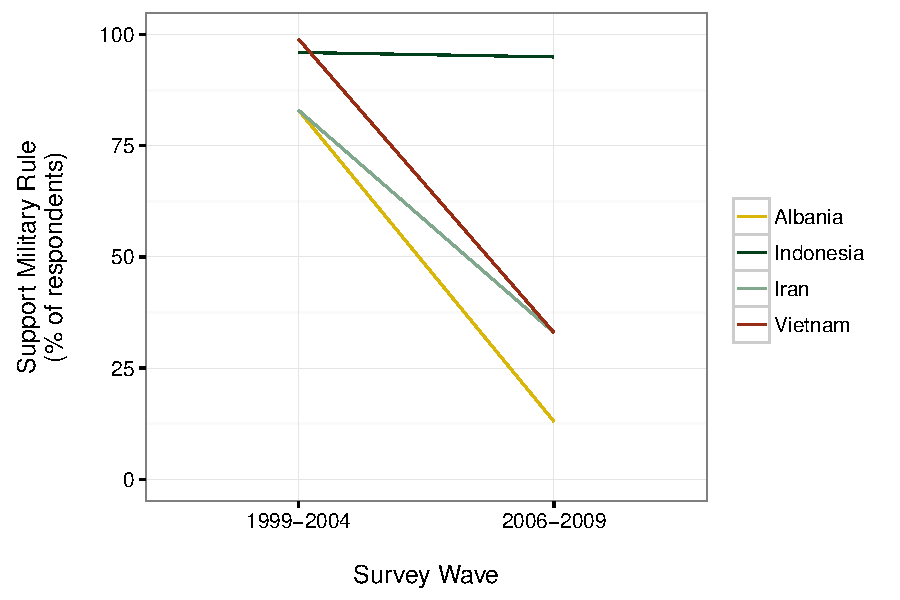
\includegraphics[scale=0.5]{img/wvs_compare.pdf}
    \end{figure}

\end{frame}

\begin{frame}

    \begin{center}
        {\large{Why did support for military rule decline so much in Albania, Iran and Vietnam in only a few years?}}

        \vspace{1cm}
    \end{center}

    Inglehart and Welzel (2005) argue that: ``If younger generations are socialized under significantly different conditions from those that shaped earlier generations, the values of the entire society will gradually change through intergenerational replacement.''

\end{frame}

\begin{frame}{More likely\ldots}

    \href{https://www.washingtonpost.com/news/monkey-cage/wp/2014/09/02/world-values-lost-in-translation/}{Kurzman (2014)} argues that it is more likely that the \textbf{question translation changed}.
{\small{
    \begin{table}
        \begin{tabular}{l p{3.5cm} p{3.5cm}}
        \hline
        & 1999-2005 & 2006-2009\\
        \hline\hline
        English & Having the military rule & Having the military rule \\

        \hline
        \end{tabular}
    \end{table}

}}

\end{frame}

\begin{frame}{More likely\ldots}

    \href{https://www.washingtonpost.com/news/monkey-cage/wp/2014/09/02/world-values-lost-in-translation/}{Kurzman (2014)} argues that it is more likely that the \textbf{question translation changed}.
{\small{
    \begin{table}
        \begin{tabular}{l p{3.5cm} p{3.5cm}}
        \hline
        & 1999-2005 & 2006-2009\\
        \hline\hline
        English & Having the military rule & Having the military rule \\

        Indonesia & Memiliki peraturan yang jelas tentang angkatan bersenjata (\textbf{having clear military rules}) & Memiliki peraturan tentang angkatan bersenjata (\textbf{having military rules})\\

        \hline
        \end{tabular}
    \end{table}

}}

\end{frame}

\begin{frame}{More likely\ldots}

    \href{https://www.washingtonpost.com/news/monkey-cage/wp/2014/09/02/world-values-lost-in-translation/}{Kurzman (2014)} argues that it is more likely that the \textbf{question translation changed}.
{\small{
    \begin{table}
        \begin{tabular}{l p{3.5cm} p{3.5cm}}
        \hline
        & 1999-2005 & 2006-2009\\
        \hline\hline
        English & Having the military rule & Having the military rule \\

        Indonesia & Memiliki peraturan yang jelas tentang angkatan bersenjata (\textbf{having clear military rules}) & Memiliki peraturan tentang angkatan bersenjata (\textbf{having military rules})\\

        Albanian & T\"{e} kesh rregulla t\"{e} ushtris\"{e} (\textbf{having military rules}) & T\"{e} kesh regjim ushtarak (\textbf{having a military regime}) \\

        \hline
        \end{tabular}
    \end{table}

}}

\end{frame}

\begin{frame}{More likely\ldots}

    \href{https://www.washingtonpost.com/news/monkey-cage/wp/2014/09/02/world-values-lost-in-translation/}{Kurzman (2014)} argues that it is more likely that the \textbf{question translation changed}.
{\small{
    \begin{table}
        \begin{tabular}{l p{3.5cm} p{3.5cm}}
        \hline
        & 1999-2005 & 2006-2009\\
        \hline\hline
        English & Having the military rule & Having the military rule \\

        Indonesia & Memiliki peraturan yang jelas tentang angkatan bersenjata (\textbf{having clear military rules}) & Memiliki peraturan tentang angkatan bersenjata (\textbf{having military rules})\\

        Albanian & T\"{e} kesh rregulla t\"{e} ushtris\"{e} (\textbf{having military rules}) & T\"{e} kesh regjim ushtarak (\textbf{having a military regime}) \\

        Vietnamese & Vai tr\`{o} c\`{u}a qu\^{a}n đội (\textbf{role of the military}) & [Unavailable] \\

        \hline
        \end{tabular}
    \end{table}

}}

\end{frame}

\begin{frame}

    \begin{center}
        \textbf{Reproducible research} practices--questionnaire and translation was available--\textbf{made it possible to find} these errors.
    \end{center}

\end{frame}

\begin{frame}{Example: Reinhart and Rogoff (2010)}

    \textbf{Background:} Reinhart and Rogoff (2010) in a highly influential study (in academics and government) found a threshold effect at 90\% Public debt/GDP and Economic Growth.

    \textbf{Original finding:}

    \begin{figure}
        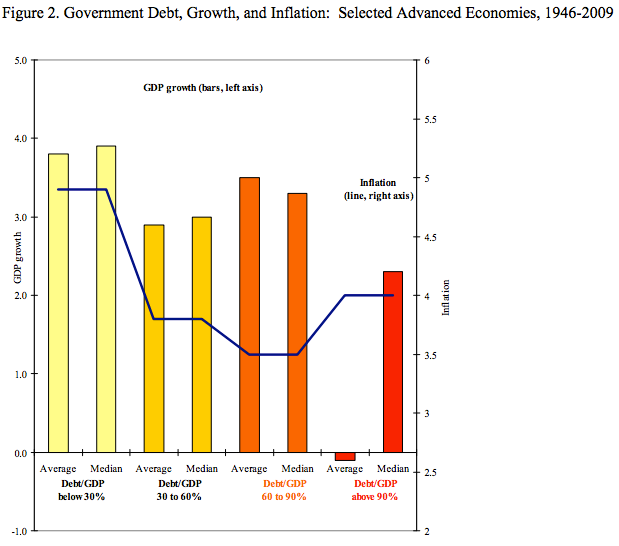
\includegraphics[scale=0.3]{img/rr_original.png}
    \end{figure}


\end{frame}

\begin{frame}

    \textbf{Replication:} But, Herndon et al. (2014) found that an \alert{Excel coding error} had dropped Australia, Austria, Belgium, Canada, and Denmark.

    \textbf{Corrected finding:}

    \begin{figure}
        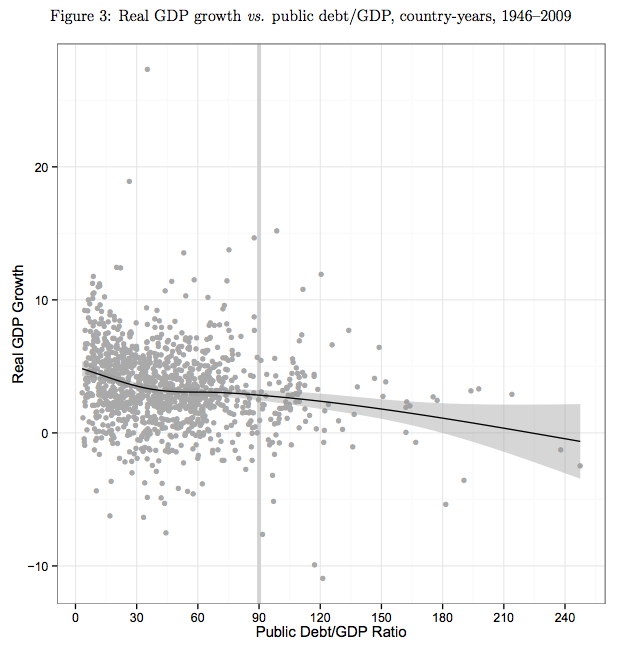
\includegraphics[scale=0.3]{img/rr_corrected.png}
    \end{figure}

\end{frame}

\begin{frame}{Example: LaCour Affair}

    \textbf{Background:} Lacour and Green (2014) found that having a conversation with a gay person had a very strong positive long-term effect on support for same-sex for marriage. This was \textbf{widely reported} in the popular press and advocacy groups began to use similar techniques.

    \textbf{Original finding:}

    \begin{figure}
        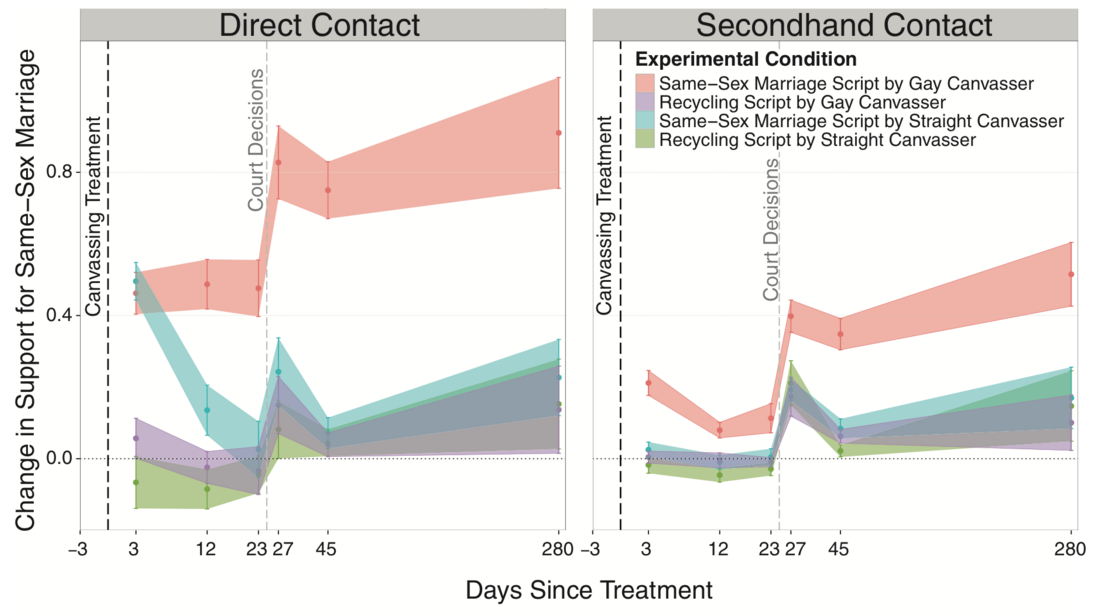
\includegraphics[scale=0.23]{img/lacour_original.png}
    \end{figure}

\end{frame}

\begin{frame}

     Broockman et al. (2015) found that LaCour had \textbf{fabricated} the survey data. (Tech details: he took someone else's survey data and added random noise to the subsequent survey ``waves''.)

     \begin{figure}
         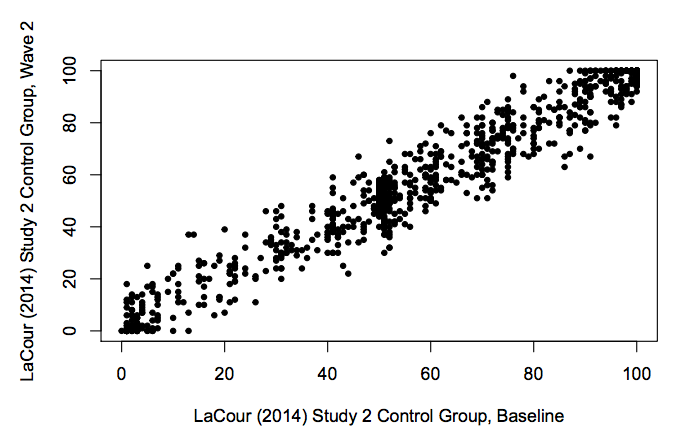
\includegraphics[scale=0.3]{img/lacour_noise.png}
     \end{figure}

\end{frame}

\begin{frame}{For science}

    Reproducible research also benefits science by:

    \begin{itemize}
        \item \textbf{Avoiding scientists wasting time} trying to understand things that does not exist.

        \vspace{0.5cm}

        \item \textbf{Avoiding effort duplication} by cutting down the time the scientific community spends gathering data/developing analytic procedures.
    \end{itemize}


\end{frame}

\section{How to do really reproducible research}

\begin{frame}

\begin{exampleblock}{Reproducible Research}
    When there is sufficient information available for independent researchers to make the same findings, using the same procedures with the \emph{same data}.
\end{exampleblock}

    \vspace{1cm}

    \begin{center}
        {\LARGE{How do we do this?}}
    \end{center}

\end{frame}

\begin{frame}{Doing reproducible research}

    {\large{Some key tips:}}

    \begin{itemize}

        \item \alert{Document everything!}

        \item All of your files should be \alert{human-readable}.

        \item \alert{From the start} of your research project, have a plan to \alert{organise}, store, and make your files accessible.

        \item Explicitly \alert{tie your files together}.
    \end{itemize}

\end{frame}


\begin{frame}{Document Everything!}

    Need to \alert{fully document} the steps we took and the rationale for these steps.

    \begin{itemize}
        \item Documentation \emph{both} in the presentation document (usually discussion of general steps) and ``appendix'' files (e.g. source code, survey questionnaires, raw data).
    \end{itemize}

\end{frame}

\begin{frame}{Document everything specifics: source code}

    It is important to record in detail the steps you used to clean and analyse your data, ideally with the original source code (e.g. SPSS Syntax or R source).

\end{frame}

\begin{frame}[fragile]{Minimal (messy) R Example}

\begin{lstlisting}
library(WDI)
library(dplyr)
library(ggplot2)
setwd('U:\\research/group_project')
women<-WDI(indicator='SG.GEN.PARL.ZS',start=1995)
women<-rename(women_in_parl=SG.GEN.PARL.ZS)
women<-filter(women,country%in%c('Algeria','Germany','Japan','Sweden'))
ggplot(women,aes(x=year,y=women_in_parl,colour=country))+
geom_line()+ylab('WomeninParliament(%)')+xlab('')+theme_bw()
\end{lstlisting}

\end{frame}

\begin{frame}{Result}

    \begin{figure}
        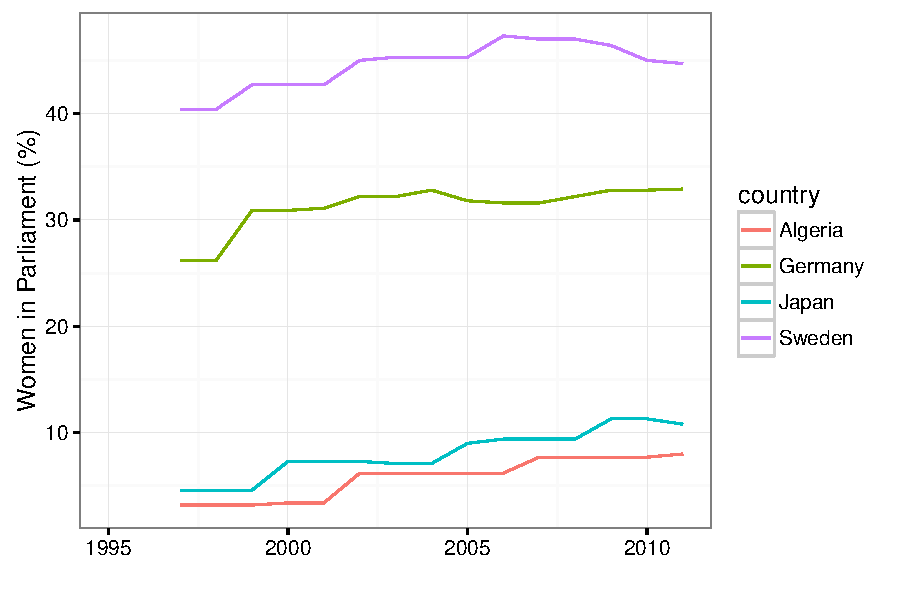
\includegraphics[scale=0.5]{img/women_compare.pdf}
    \end{figure}

\end{frame}

\begin{frame}{Human-readable}

    Even files that you intend a computer to run should be \textbf{human-readable}.

    \vspace{1.5cm}

    So that another person (and yourself in the future) can \textbf{understand} what you did, even if the computer program no longer exists (helps \textbf{future-proof} your work).

    \vspace{0.5cm}

    So \ldots

\end{frame}

\begin{frame}{Formatting and Comment characters}

    Write your source code with the \textbf{intention} that it will be read by a person.

    \begin{itemize}
        \item Use a \textbf{consistent style} (just as you would in a presentation document).

        \item Use \alert{comment characters} that allow you to write information that humans can read and the computer will ignore.

            \begin{itemize}
                \item R comment character: \texttt{\#}
                \item SPSS comment character: \texttt{*}
            \end{itemize}
    \end{itemize}


\end{frame}

\begin{frame}[fragile]{Minimal (human-readable) R Example (1)}

\begin{lstlisting}
#########################
# Gather women in parliament data from WDI and plot subset
# Christopher Gandrud
#########################

# Load required packages
library(WDI)
library(dplyr)
library(ggplot2)

# Set working directory. Changed as needed
setwd('U:\\research/group_project')

# Download women in parliament data from
# World Bank Development indicators
# from 1995. Indicator ID = SG.GEN.PARL.ZS
women <- WDI(indicator = 'SG.GEN.PARL.ZS', start = 1995)
\end{lstlisting}

\end{frame}

\begin{frame}[fragile]{Minimal (human readable) R Example (2)}

\begin{lstlisting}
# Clean up: (1) rename women in parliament indicator,
# (2) select data from Algeria, Germany, Japan, and Sweden
women <- rename(women, women_in_parl = SG.GEN.PARL.ZS)
women <- filter(women, country %in%
                c('Algeria', 'Germany', 'Japan', 'Sweden'))

# Create a comparative line plot of the data
ggplot(women, aes(x = year, y = women_in_parl, colour = country)) +
geom_line() +
ylab('Women in Parliament (%)') + xlab('') +
theme_bw()
\end{lstlisting}

\end{frame}


\begin{frame}[fragile]{Minimal SPSS Example}

\begin{lstlisting}
* Load data from 'employee data.sav' file in the C drive.
GET FILE='C:\program files\spss\employee data.sav'.

* Find frequencies of jobcat variable and order
FREQUENCIES
    VARIABLES=jobcat
    ORDER=ANALYSIS.
\end{lstlisting}

\end{frame}

\begin{frame}{Organise your files into an understandable hierarchy}

    Start your research with a plan to to organise, store, and make your files available.

    \begin{figure}
        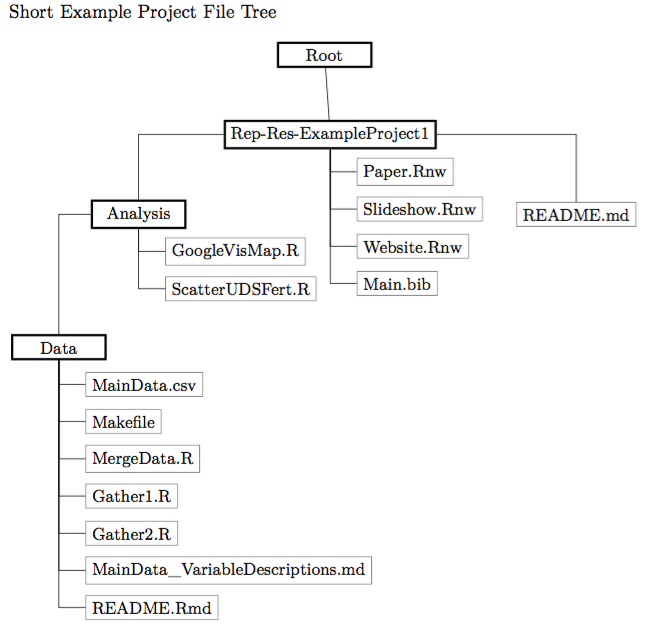
\includegraphics[scale=0.3]{img/file_tree.png}
    \end{figure}

{\tiny{Gandrud (2015)}}

\end{frame}

\begin{frame}{File ties}

    Your files should be \textbf{tied} together in a \textbf{documented} and \textbf{understandable} way, so that others (and your future) self will understand your research process.

\end{frame}

\begin{frame}

    \begin{figure}
        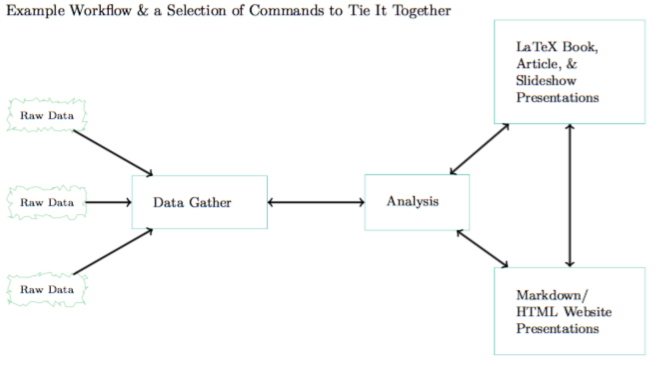
\includegraphics[scale=0.35]{img/workflow.png}
    \end{figure}
{\tiny{Gandrud (2015, 21)}}


Note, we don't cover all of the tools to do all of this in this course.
\end{frame}


\begin{frame}[fragile]{Minimal R Example}

\begin{lstlisting}
#########################
# Gather women in parliament data from WDI and save locally
# Christopher Gandrud
#########################

# Load required packages
library(WDI)
library(dplyr)
library(rio)

# Set working directory. Changed as needed
setwd('U:\\research/group_project')

# Download women in parliament data from
# World Bank Development indicators
# from 1995. Indicator ID = SG.GEN.PARL.ZS
women <- WDI(indicator = 'SG.GEN.PARL.ZS', start = 1995)

# Save data in CSV format
export(women, file = 'data/women_in_parl_wdi.csv')
\end{lstlisting}

\end{frame}


\begin{frame}{The reproducible research ideal}

    Ideally, data gathering, analysis, and presentation can be \textbf{dynamically} linked.

    \vspace{1cm}

    We don't cover these tools in this class, but FYI, they go by names such as RMarkdown and Sweave.

\end{frame}

\begin{frame}{This \ldots}

    \begin{figure}
            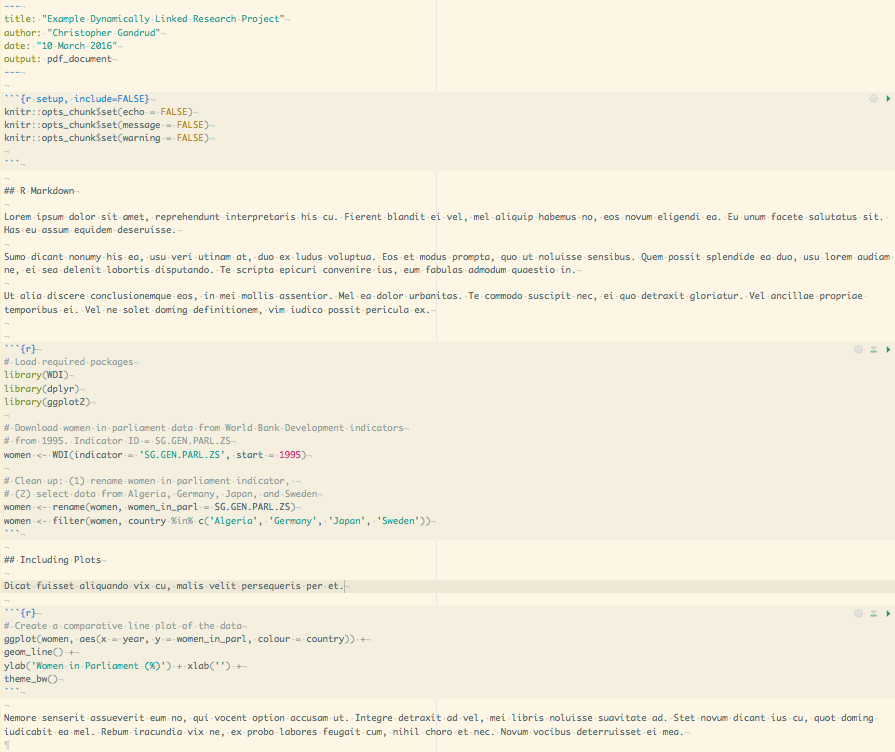
\includegraphics[scale=0.3]{img/rmarkdown_source.png}
    \end{figure}

\end{frame}

\begin{frame}{Is all you need to create this \ldots}

    \begin{figure}
            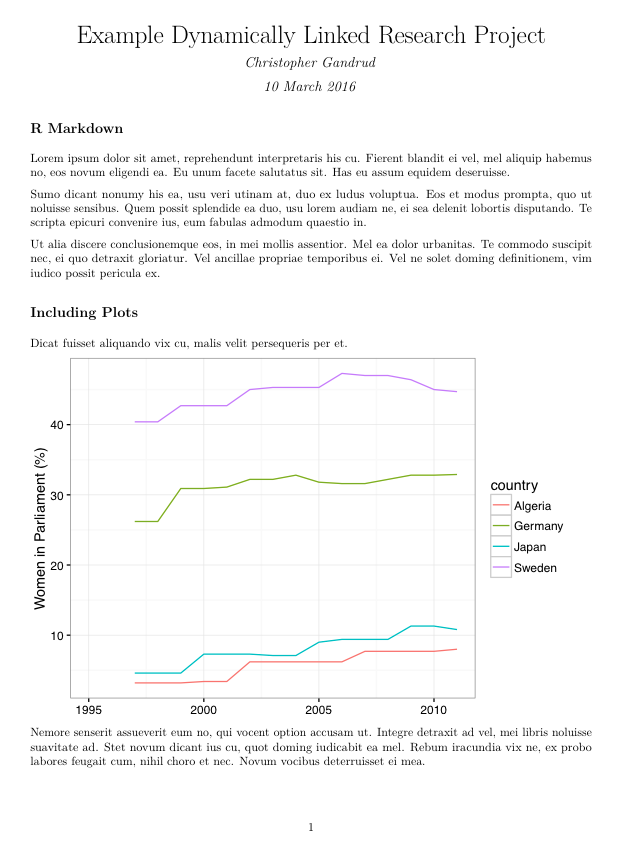
\includegraphics[scale=0.3]{img/rmarkdown_result.png}
    \end{figure}

\end{frame}

\begin{frame}{Your group projects}

    Your project should be \textbf{reproducible}.

    \begin{itemize}
        \item Your paper should have clear descriptions of your measurement instrument
        \begin{itemize}
            \item Survey: questionnaire
            \item Content analysis: coding scheme
            \item Composite indicators: original variables and how they were aggregated
        \end{itemize}

        \item A complete account of your data
        \begin{itemize}
            \item Including as much raw data (e.g. texts for content analysis, data sets for surveys) as possible with instructions (detailed descriptions and syntax where possible) for how you accessed/set up, cleaned and analysed it
            \item You should submit separate file types as appendices to your report
        \end{itemize}

    \end{itemize}

\end{frame}




\end{document}
